\documentclass[tikz,border=12pt]{standalone}
\usepackage[T1]{fontenc}
\usepackage{tgheros}
\usepackage{sfmath}
\usepackage{amsmath}
\usepackage{fontawesome5}
\usepackage{tikz}
\usetikzlibrary{arrows.meta,positioning,shapes.geometric,fit,backgrounds,calc}
\usepackage{xcolor}

\renewcommand{\familydefault}{\sfdefault}

% Harvard Crimson & ETH Zurich Academic Semantic Palette
\definecolor{harvardcrimson}{HTML}{A51C30}
\definecolor{ethdarkblue}{HTML}{1F407A}
\definecolor{ethblue}{HTML}{215CAF}
\definecolor{ethpetrol}{HTML}{007A87}
\definecolor{ethbronze}{HTML}{B87333}
\definecolor{ethpurple}{HTML}{5B4B8A}
\definecolor{ethslate}{HTML}{475569}
\definecolor{darkslate}{HTML}{0F172A}
\definecolor{cardbg}{HTML}{F8FAFC}
\definecolor{cardborder}{HTML}{CBD5E1}
\definecolor{linegray}{HTML}{E2E8F0}

\begin{document}
\begin{tikzpicture}[
  font=\sffamily,
  >=Stealth,
  columncard/.style={
    draw=cardborder,
    fill=cardbg,
    rounded corners=5pt,
    line width=0.8pt,
    text width=1.56in,
    minimum height=4.05in,
    inner sep=6.5pt,
    align=left,
    anchor=north
  }
]

  % Top Title Banner (width 9.04in, centered at 4.60in)
  \node[draw=ethdarkblue, fill=ethdarkblue!5, rounded corners=5pt, line width=0.9pt, text width=9.04in, inner sep=7pt, align=center] (title) at (4.60in, 0) {
    {\normalsize\bfseries\color{ethdarkblue}\faIcon{shield-alt}\;\; THE PHYSICAL CONSTRAINTS OF EMBODIED ARTIFICIAL INTELLIGENCE}\\[2pt]
    {\scriptsize\color{ethslate}What the Physical Universe Demands of Any Proposed Motor Command}
  };

  % --- CARD 1: Time & Freshness (center = 0.92in) ---
  \node[columncard, draw=ethblue!80] (col1) at (0.92in, -0.65in) {
    {\footnotesize\bfseries\color{ethblue}\faIcon{clock}\; 1. Time \& Freshness}\\[3pt]
    {\tiny\itshape\color{ethslate}Is the evidence still true?}\\[5pt]
    {\scriptsize\textbf{Governing Physics:}}\\[1pt]
    {\tiny Information Age: $\Delta t = t_{\text{act}} - t_{\text{sens}}$\\
    World Deadline: $\tau_{\text{world}}$\\
    Uncertainty: $\sigma(t) = \sigma_0 + v\Delta t$}\\[6pt]
    \rule{0.95\linewidth}{0.3pt}\\[4pt]
    {\scriptsize\textbf{Systems Metrics:}}\\[2pt]
    {\tiny $\bullet$ Freshness Wall $\Delta t_{\text{wall}}$\\
    $\bullet$ Tail Latency ($P_{99}, P_{99.9}$)\\
    $\bullet$ Latest-Frame Sampling\\
    $\bullet$ Action Chunking ($H$ steps)}\\[6pt]
    \rule{0.95\linewidth}{0.3pt}\\[4pt]
    {\scriptsize\textbf{\color{ethblue}Reaches:}}\\[1pt]
    {\tiny All cognitive stages.}\\[4pt]
    {\scriptsize\textbf{\color{ethblue}Failure Mode:}}\\[1pt]
    {\tiny Stale-state collapse; open-loop drift during latency spikes.}
  };

  % --- CARD 2: Inertia & Stopping (center = 2.76in) ---
  \node[columncard, draw=ethbronze!90] (col2) at (2.76in, -0.65in) {
    {\footnotesize\bfseries\color{ethbronze}\faIcon{tachometer-alt}\; 2. Inertia \& Stopping}\\[3pt]
    {\tiny\itshape\color{ethslate}Can the machine still stop?}\\[5pt]
    {\scriptsize\textbf{Governing Physics:}}\\[1pt]
    {\tiny Momentum: $\mathbf{p} = m\mathbf{v}$\\
    Kinetic Energy: $E_k = \frac{1}{2}m v^2$\\
    Braking Decel: $a_{\text{max}} \le \mu g$}\\[6pt]
    \rule{0.95\linewidth}{0.3pt}\\[4pt]
    {\scriptsize\textbf{Systems Metrics:}}\\[2pt]
    {\tiny $\bullet$ Stopping Envelope $d_{\text{stop}}$\\
    $\bullet$ Linear Reaction: $v \cdot \Delta t$\\
    $\bullet$ Quadratic Brake: $\frac{v^2}{2a_{\text{max}}}$\\
    $\bullet$ Clearance Barrier: $d_{\text{clear}}$}\\[6pt]
    \rule{0.95\linewidth}{0.3pt}\\[4pt]
    {\scriptsize\textbf{\color{ethbronze}Reaches:}}\\[1pt]
    {\tiny Perception, Memory, Planning, Execution.}\\[4pt]
    {\scriptsize\textbf{\color{ethbronze}Failure Mode:}}\\[1pt]
    {\tiny Kinetic overrun; obstacle collision during braking.}
  };

  % --- CARD 3: Actuation Limits (center = 4.60in) ---
  \node[columncard, draw=harvardcrimson!80] (col3) at (4.60in, -0.65in) {
    {\footnotesize\bfseries\color{harvardcrimson}\faIcon{cogs}\; 3. Actuation Limits}\\[3pt]
    {\tiny\itshape\color{ethslate}How fast may commands change?}\\[5pt]
    {\scriptsize\textbf{Governing Physics:}}\\[1pt]
    {\tiny Torque Rate: $\dot{\boldsymbol{\tau}} = d\boldsymbol{\tau}/dt$\\
    Jerk: $\dddot{\mathbf{q}} = d^3\mathbf{q}/dt^3$\\
    Shear: $\sigma = \boldsymbol{\tau}/W_p \le \sigma_{\text{yield}}$}\\[6pt]
    \rule{0.95\linewidth}{0.3pt}\\[4pt]
    {\scriptsize\textbf{Systems Metrics:}}\\[2pt]
    {\tiny $\bullet$ Torque Rate Clamp\\
    $\bullet$ $\mathcal{C}^2$ Jerk-Continuous Splines\\
    $\bullet$ Backlash \& Compliance\\
    $\bullet$ Torque Saturation}\\[6pt]
    \rule{0.95\linewidth}{0.3pt}\\[4pt]
    {\scriptsize\textbf{\color{harvardcrimson}Reaches:}}\\[1pt]
    {\tiny Planning and Execution.}\\[4pt]
    {\scriptsize\textbf{\color{harvardcrimson}Failure Mode:}}\\[1pt]
    {\tiny Gearbox tooth shear; resonance chatter.}
  };

  % --- CARD 4: Energy & Thermal (center = 6.44in) ---
  \node[columncard, draw=ethpurple!85] (col4) at (6.44in, -0.65in) {
    {\footnotesize\bfseries\color{ethpurple}\faIcon{thermometer-half}\; 4. Energy \& Thermal}\\[3pt]
    {\tiny\itshape\color{ethslate}What does it cost to sustain?}\\[5pt]
    {\scriptsize\textbf{Governing Physics:}}\\[1pt]
    {\tiny Joule Heat: $C_{\text{th}}\dot{T} = I^2R - \frac{\Delta T}{R_{\text{th}}}$\\
    Continuous: $I_{\text{cont}} = \sqrt{\Delta T_{\text{max}} / (R R_{\text{th}})}$\\
    Junction: $T_j \to$ DVFS throttle}\\[6pt]
    \rule{0.95\linewidth}{0.3pt}\\[4pt]
    {\scriptsize\textbf{Systems Metrics:}}\\[2pt]
    {\tiny $\bullet$ $I^2t$ Accumulation Clamp\\
    $\bullet$ Shared Power Rail Budget\\
    $\bullet$ Thermal-State Provenance\\
    $\bullet$ Extrinsic Calibration Drift}\\[6pt]
    \rule{0.95\linewidth}{0.3pt}\\[4pt]
    {\scriptsize\textbf{\color{ethpurple}Reaches:}}\\[1pt]
    {\tiny Mounts, Accelerators, Motors.}\\[4pt]
    {\scriptsize\textbf{\color{ethpurple}Failure Mode:}}\\[1pt]
    {\tiny Winding burnout; silent clock throttle past deadline.}
  };

  % --- CARD 5: Silicon Determinism (center = 8.28in) ---
  \node[columncard, draw=ethpetrol!90] (col5) at (8.28in, -0.65in) {
    {\footnotesize\bfseries\color{ethpetrol}\faIcon{microchip}\; 5. Silicon Determinism}\\[3pt]
    {\tiny\itshape\color{ethslate}Will the chip respond on time?}\\[5pt]
    {\scriptsize\textbf{Governing Physics:}}\\[1pt]
    {\tiny Crossbar Saturation: UMA DRAM\\
    Ingestion Tax: DMA vs NPU\\
    SRAM Mailbox: Lock-Free Ring}\\[6pt]
    \rule{0.95\linewidth}{0.3pt}\\[4pt]
    {\scriptsize\textbf{Systems Metrics:}}\\[2pt]
    {\tiny $\bullet$ Pre-Inference Bus Tax\\
    $\bullet$ Heterogeneous Coherency\\
    $\bullet$ Zero-Heap Real-Time Rule\\
    $\bullet$ Hardware Watchdog Leases}\\[6pt]
    \rule{0.95\linewidth}{0.3pt}\\[4pt]
    {\scriptsize\textbf{\color{ethpetrol}Reaches:}}\\[1pt]
    {\tiny All compute substrates.}\\[4pt]
    {\scriptsize\textbf{\color{ethpetrol}Failure Mode:}}\\[1pt]
    {\tiny Memory bus starvation; non-deterministic heap pause.}
  };

  % Bottom Summary Bar (width 9.04in, centered at 4.60in)
  \node[draw=ethdarkblue, fill=white, rounded corners=4pt, line width=0.8pt, text width=9.04in, inner sep=6pt, align=center] at (4.60in, -4.95in) {
    {\scriptsize\textbf{\color{ethdarkblue}\faIcon{check-circle}\; THE CO-DESIGN INVARIANT:} Every cognitive action proposed by software must satisfy all physical constraints before motor inverters are energized.}
  };

\end{tikzpicture}
\end{document}
